  \section{Bio2RDF}
  \label{sec:bio2rdf}
  
  \initial{B}\textit{io2RDF} is an open source project that uses semantic web\
  technologies to build and provide the largest network of Linked Data for the\
  Life Sciences. It defines a set of simple conventions to create\
  RDF\textsuperscript{\ref{sec:rdf}}\
  compatible Linked Data from a diverse set of heterogeneously formatted\
  sources obtained from multiple data providers. Bio2RDF is the culmination\
  of efforts towards addressing the pressing need for a global multisite\
  search engine. It is defined as a system that is able to query and connect\
  different databases available on the Internet~\citep{belleau_bio2rdf:_2008}.\\
    
  \begin{figure}[ht!]
    \centering
    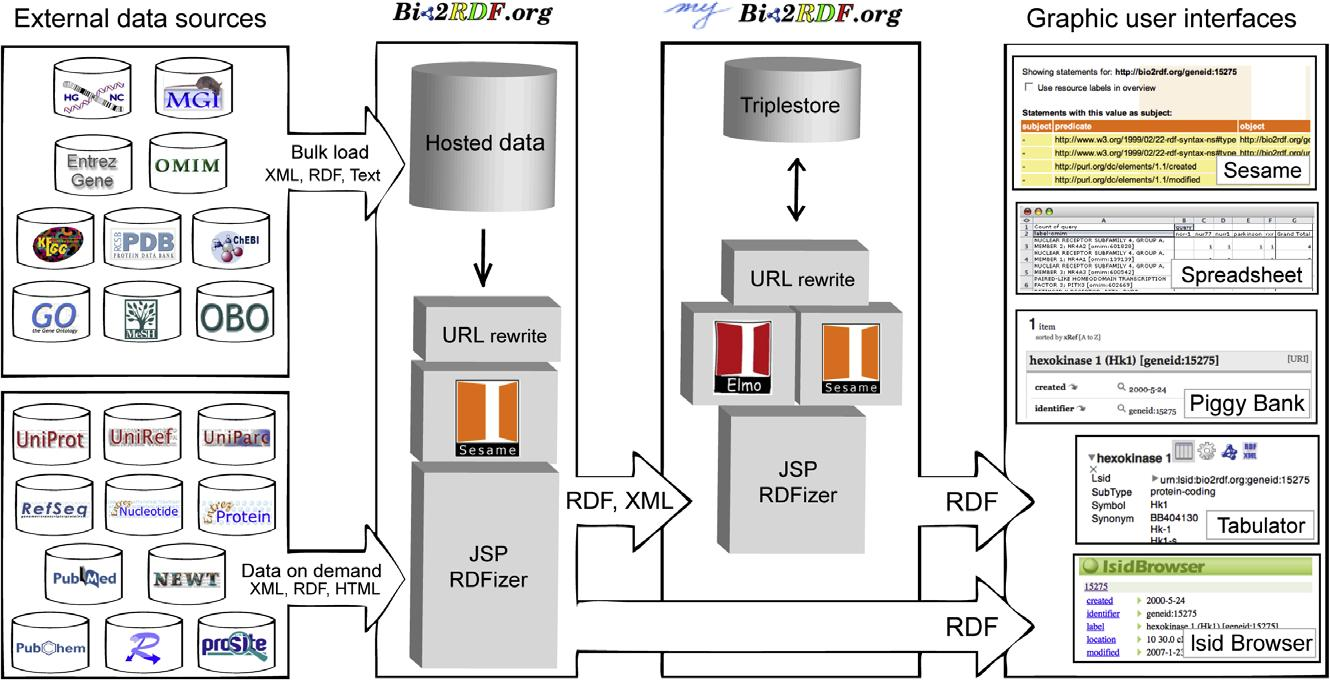
\includegraphics[scale=0.30]{bio2rdf_architecture.jpg}
    \caption{Bio2RDF knowledge system framework\
    architecture~\citep[Fig.~1]{belleau_bio2rdf:_2008}}
    \label{fig:bio2rdf_architecture}
  \end{figure}  

  \noindent Bio2RDF uses RDF documents and a\
  list of rules\
  (\emph{Banff Manifesto\footnote{\url{http://sourceforge.net/apps/mediawiki/bio2rdf/index.php?title=Banff_Manifesto}}})\
  to create URIs that will produce linked data:
  \begin{itemize}
    \itemindent3em
    \itemsep0ex
    \item [\textbf{Rule 1:}] URI's are normalized and dereferencable
    \item [\textbf{Rule 2:}] Authoritative public namespaces are used 
    \item [\textbf{Rule 3:}] Mandatory predicates are used
    \item [\textbf{Rule 4:}] Blank nodes are forbidden
    \item [\textbf{Rule 5:}] RDFizer programs are open source
    \item [\textbf{Rule 6:}] Deference-able ontologies
  \end{itemize}
  Figure~\ref{fig:bio2rdf_architecture} shows a schematic description\
  of the Bio2RDF architecture. All external data sources, in different formats\
  (XML, Text, ASN.1, KGML and RDF), are listed on the left part. Data is then\
  made accessible either on the Bio2RDF.org server or on demand from the\
  original source. The myBio2RDF application contains an rdfizer program\
  and a servlet that answers Bio2RDF HTTP requests by formulating\
  SPARQL\textsuperscript{\ref{sec:sparql}} endpoints~\citep{callahan_bio2rdf_2013}.\\
  
  \subsection{Naming Convention}
  Bio2RDF entities are named as follows:
  \begin{quote}
    \url{http://bio2rdf.org/namespace:identifier}
  \end{quote}
  \noindent where, \emph{namespace} is the preferred short name of a\
  biological dataset and \emph{identifier} is the unique string used\
  by the source provider to identify the given record. For example,\
  HUGO Gene Nomenclature Committee identifies the human prostaglandin\
  E synthase gene (PIG12) with the accession number `9599'. This\
  dataset's namespace is ``hgnc'' in Bio2RDF's dataset\
  registry\footnote{\url{https://docs.google.com/spreadsheet/ccc?key=0AnGgKfZdJasrdElfQzRWWWhKUFR0UnRpeG14NGZRS2c}}\
  and the corresponding Bio2RDF IRI is:~\url{http://bio2rdf.org/hgnc:9599}\
  There are over 1800 such namespaces.
  
  \subsection{Bio2RDF Dataset Provenance Model}
  Provenance data for each Bio2RDF dataset is stored in a separate named\
  graph in each corresponding SPARQL endpoint. The provenance graph URI\
  follows the pattern:
  \begin{quote}
    \url{http://bio2rdf.org/bio2rdf-[dataset]-provenance}    
  \end{quote}
  \noindent where, `dataset' is the preferred short name (or prefix) for a given source\
  dataset as extracted from the Life Science Registry\footnote{Hosted by Bio2RDF\
  at \url{https://docs.google.com/spreadsheet/ccc?key=0AmzqhEUDpIPvdFR0UFhDUTZJdnNYdnJwdHdvNVlJR1E}}.\\
  
  \begin{figure}[ht!]
    \centering
    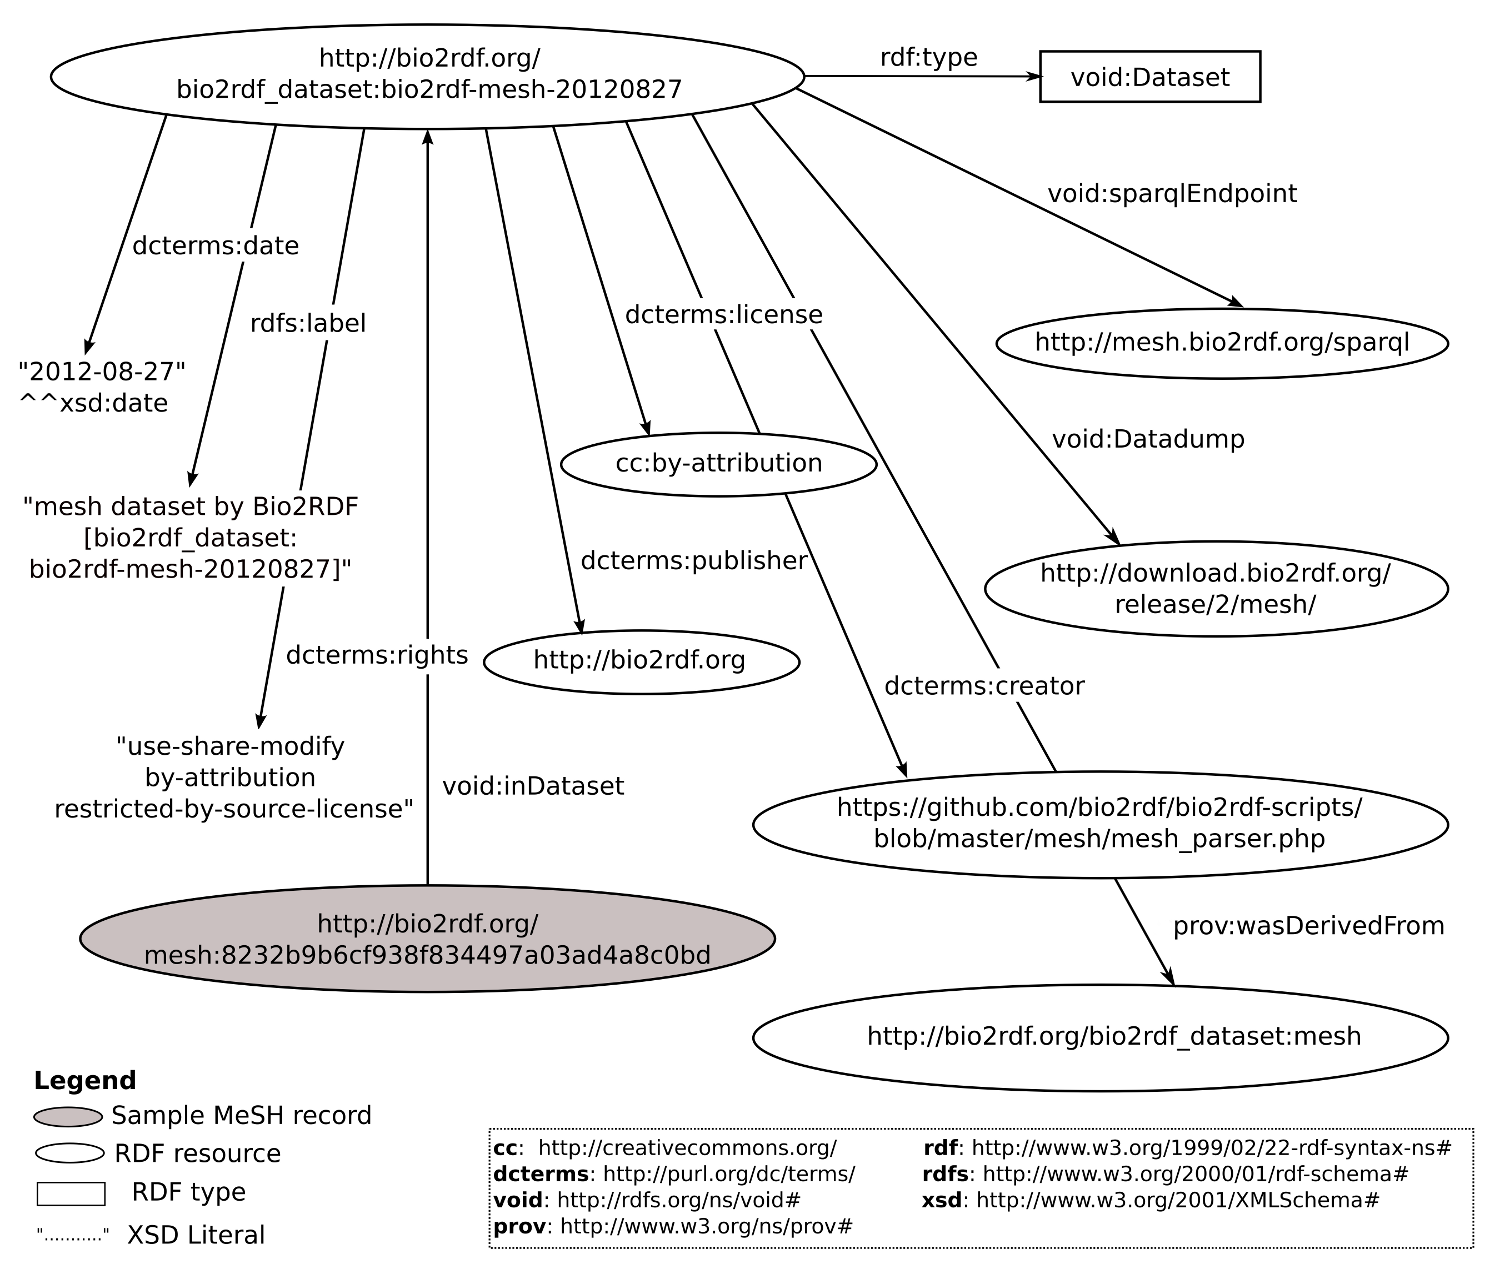
\includegraphics[scale=2.80,trim=1 1 1 1,clip]{bio2rdf_provenance.png}
    \caption{Bio2RDF Provenance Graph for the NLM Medical Subject Headings (MeSH)\
    architecture~\citep{bio2rdf_wiki_bio2rdf_2013}}
    \label{fig:bio2rdf_provenance}
  \end{figure}  
  
  \noindent For example, the ``NLM Medical Subject Headings (MeSH)'' dataset\
  provenance graph makes use of \url{http://bio2rdf.org/bio2rdf-mesh-provenance}\
  as its graph URI. Bio2RDF's provenance model uses the W3C Vocabulary of\
  Interlinked Datasets (VoID), the Provenance vocabulary (PROV) and\
  Dublin Core vocabulary.\
  Each dataset provenance object has a unique IRI and label based on the\
  dataset name and creation date. For example,\
  \url{http://bio2rdf.org/bio2rdf_dataset:bio2rdf-mesh-20120827}.\
  An example provenance graph for the MeSH dataset can be seen in Figure~\ref{fig:bio2rdf_provenance}.\
  Note that each subject IRI in the dataset is linked the date-unique dataset\
  IRI that is part of the provenance record using the VoID `inDataset' predicate.\
  Other important features of the provenance record include the use of the Dublin\
  Core `creator' term to link a dataset to the script on Github that was used to\
  generate it, the VoID predicate `sparqlEndpoint' to point to the dataset SPARQL\
  endpoint, and VoID predicate `dataDump' to point to the data download URL.\\
  
  \noindent Although Bio2RDF facilitates integration of and programmatic access\
  to otherwise heterogeneous datasets (in both, content and format), a complete\
  syntactic and semantic normalization across numerous datasets has yet to be\
  fully realized. Works of~\citep{ansell_model_2011, callahan_ontology-based_2013, castro_biotea:_2013}\
  demonstrate better and improved models of resolving queries to the Bio2RDF datasets.\\
